\section{Estimating road speeds}
\label{sec:vehicle_speeds}

Now that we have estimated the necessary vehicle states and their respective trajectories, we can infer each vehicle's \emph{average speed} along road segment $\ell$ of its current route, $\Vtt_{\ell}$. These estimates are later used to update the \emph{road network state} (\cref{cha:network_model}) and ultimately estimate arrival times (\cref{cha:prediction}).


Estimation of average road speed is performed by first computing the \emph{travel time} along each road segment as the bus traverses the network. To do so, we record the time when the vehicle starts and ends each segment, $\Vsegstart_\ell$ and $\Vsegend_\ell$, respectively, and take the difference to obtain the travel time in seconds. By using a particle filter, we record these values for each particle as it is transitioned to each new state. Finally, transforming to average speed uses the length of the segment, $\Tseglen_\ell$, in meters, and the standard speed formula ($\text{speed} = \frac{\text{distance}}{\text{time}}$):
\begin{equation}
\label{eq:vehicle_avg_speed}
\Vtt\vi_\ell = \frac{\Tseglen_\ell}{{\Vsegend}\vi_\ell - {\Vsegstart}\vi_\ell}.
\end{equation}


Since estimating \cref{eq:vehicle_avg_speed} is straightforward for each particle, the posterior distribution of the vehicle's average travel time along segment $\ell$, given all observations up to and including time $\Vtime_k$, is approximated using the Dirac delta measure,
\begin{equation}
\label{eq:pf_speed_dist}
p(\Vtt_\ell \cond{} \Vobs_{1:k}) \approx
\sum_{i=1}^\Np \Pwt_k \DiracMeasure{\Vtt\vi_\ell}{\Vtt_\ell}.
\end{equation}
In situations where only some particles have completed travel along a segment, the application waits until the next iteration to re-check that all particles have completed it and, if so, the average speed is calculated.


\subsection{Simulation study}
\label{eq:pf_simulation_study}

To assess the accuracy of the models presented in \cref{sec:vehicle_model}, vehicle simulations were performed with known road speeds while tracking the vehicle along the route. Three different sampling methods were used to obtain observations:
\begin{itemize}
\item uniform sampling with 10~second intervals;
\item uniform sampling with 30~second intervals; and
\item non-uniform sampling at nodes.
\end{itemize}
As mentioned in \cref{sec:vp_data}, the last of these is, in fact, a common feature of the Auckland Transport data; we discuss the complications further in \cref{sec:pf_implementation}. In each simulation, we implemented the three variations of the transition function: $\Vtrans_{A1}$, $\Vtrans_{A2}$, and $\Vtrans_{A3}$.


The posterior mean travel time was used to examine and compare the estimation accuracy of the models, which is simple to calculate from the particle filter estimates of travel time using the weighted mean of the sample (\cref{app:particle-summaries}):
\begin{equation}
\label{eq:pf_travel_time_mean}
\bar\Vtt_\ell =
\E{\Vtt_\ell | \Vobs_{1:k}} =
\sum_{i=1}^\Np \Pwt_k \Vtt\vi_\ell.
\end{equation}


To evaluate and compare the estimation performance of the models, we use \gls{rmse} and \gls{mae}:
\begin{align}
\label{eq:pf_rmse}
\text{RMSE} &= \sqrt{\frac{1}{N}\sum_{n=1}^N \left(X_a - \hat X_n\right)^2}, \\
\label{eq:pf_mae}
\text{MAE} &= \frac{1}{N}\sum_{n=1}^N \left|X_a - \hat X_n\right|,
\end{align}
where $X_a$ is the true travel time and $X_n:n=1,\ldots,N$ are the model estimates.


\subsubsection{Simulation A: general vehicle model}
\label{sec:vehicle_sim_A}





The simulated data, shown in \cref{fig:sim1_graph}, uses the transition model described by $\Vtrans_{A3}$ to simulate a vehicle trajectory ignoring bus stops. Observations are obtained using three sampling methods: uniform sampling with high and low frequency, and non-uniform sampling, which is more in line with how the Auckland Transport data is collected.


The goal of the simulation is to estimate the vehicle's average speed along several road segments, as well as the associated uncertainty. The simulation was performed in \Rstats{} \citep{rcore} using $\Np = 2000$ particles per vehicle, and so the implementation is slightly different from the \Cpp{} one defined in \cref{sec:pf_implementation}.

\begin{knitrout}\small
\definecolor{shadecolor}{rgb}{0.969, 0.969, 0.969}\color{fgcolor}\begin{figure}
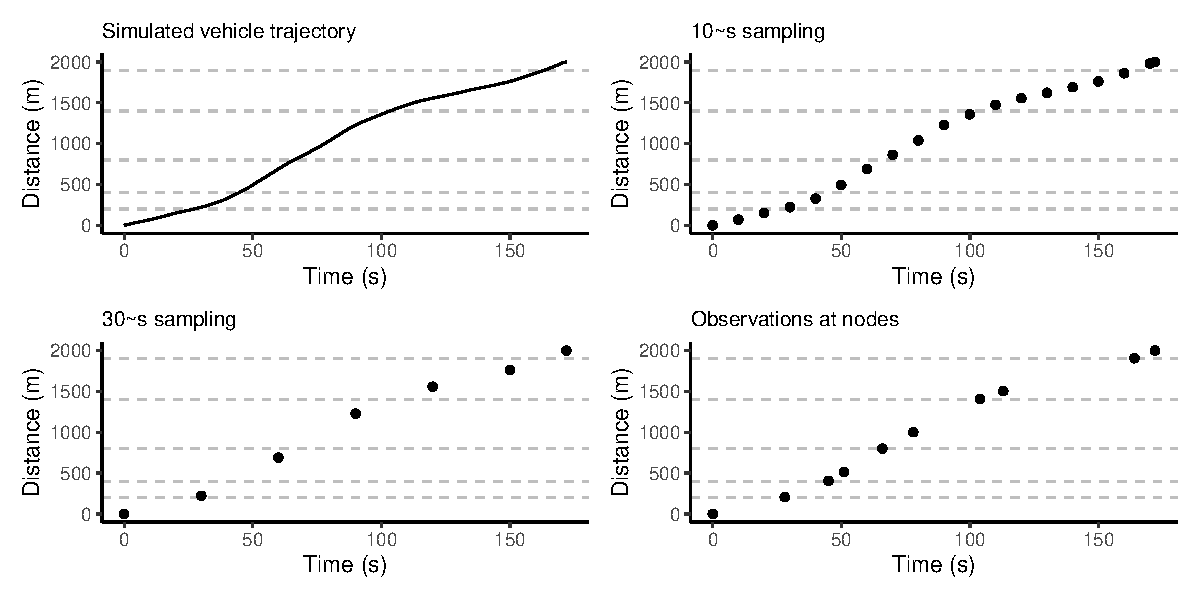
\includegraphics[width=\linewidth]{figure/sim1_graph-1} \caption[Vehicle trajectory with sampled observations for simulation A]{A simulated vehicle trajectory (top left) for simulation A along five road segments (dashed grey lines). Observations are sampled using three techniques (see text).}\label{fig:sim1_graph}
\end{figure}


\end{knitrout}

\begin{knitrout}\small
\definecolor{shadecolor}{rgb}{0.969, 0.969, 0.969}\color{fgcolor}\begin{figure}
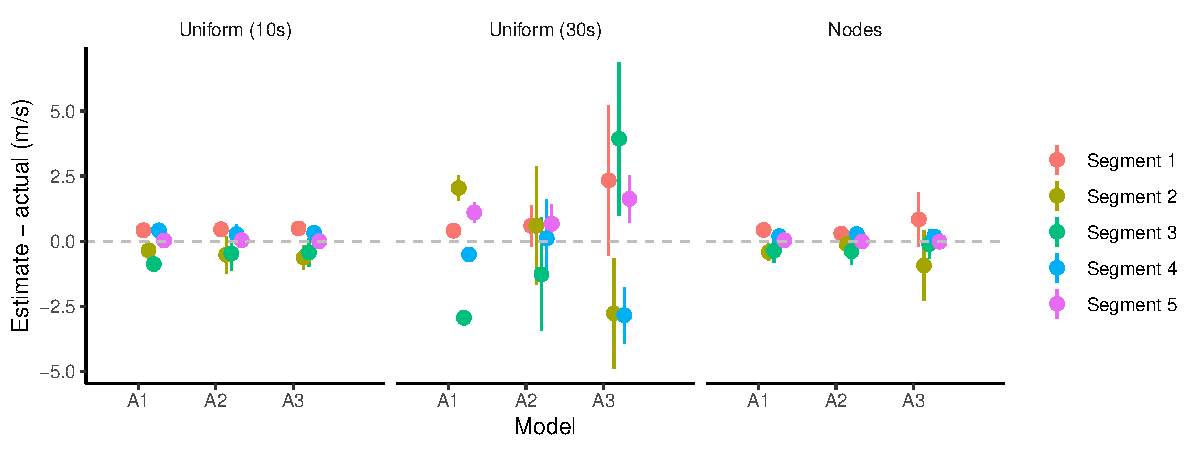
\includegraphics[width=\linewidth]{figure/sim1_pf-1} \caption[Results for simulation A]{Simulation A results for the three models (A1, A2, A3) applied to the data from three sampling methods using $\Np=2000$ particles. Shown is the travel time prediction error along with its standard deviation.}\label{fig:sim1_pf}
\end{figure}


\end{knitrout}


The results of the simulation applied to the data displayed in \cref{fig:sim1_graph} is shown in \cref{fig:sim1_pf}. Under the high-frequency uniform sampling method, all models perform similarly with high precision (the errors are all close to zero) and accuracy (the uncertainty is small enough that the error bars are barely visible). For the low-frequency sampling, however, model A2 shows slightly better precision than A1 and A3. Finally, for sampling at nodes, the models all perform similarly.



To further examine the comparative performance of the models, we repeated the simulation 100~times using the same segments and sampling points, but varying the underlying trajectory of the vehicle, with the results displayed in \cref{fig:sim1_pf_full}. Models A1 and A2 have better accuracy than A3. Most obviously, however, is that the sampling rate significantly affects accuracy. An overall comparison of \gls{rmse} and \gls{mae} are displayed in \cref{tab:sim1_pf_full}, which affirms the findings that A3 is less accurate than the other methods  (except under high-frequency sampling where they all perform similarly).


\begin{knitrout}\small
\definecolor{shadecolor}{rgb}{0.969, 0.969, 0.969}\color{fgcolor}\begin{figure}
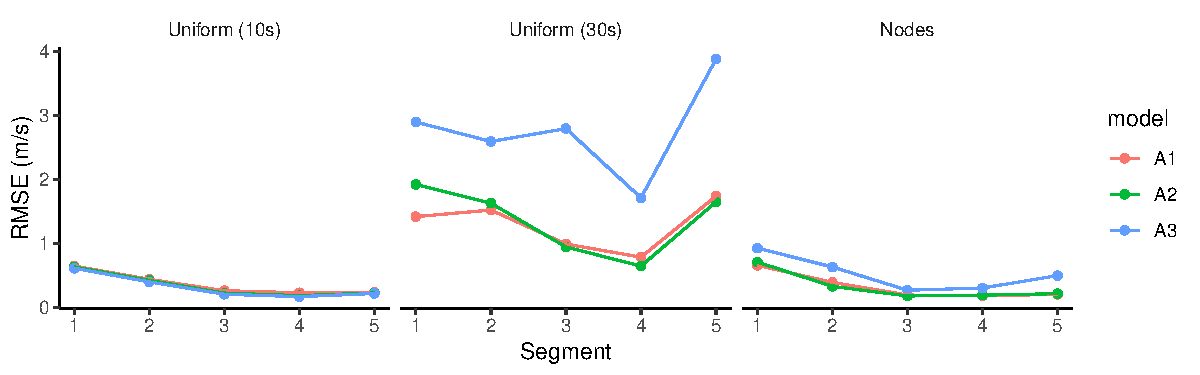
\includegraphics[width=\linewidth]{figure/sim1_pf_full-1} \caption[Results for simulation A replicated 100~times]{Speed estimation results for 100 simulations. In each the vehicle trajectory was simulated using a different seed and speed estimated by the mean of the particles, which is compared to the true speed using \gls{rmse}.}\label{fig:sim1_pf_full}
\end{figure}

\begin{table}

\caption{\label{tab:sim1_pf_full}RMSE and MAE of average speed estimation for simulation A for three models and three sampling techniques.}
\centering
\fontsize{8}{10}\selectfont
\begin{tabular}[t]{llrr}
\toprule
Sampling method & Model & RMSE (m/s) & MAE (m/s)\\
\midrule
Uniform (10s) & A1 & 0.40 & 0.27\\
 & A2 & 0.38 & 0.26\\
 & A3 & 0.36 & 0.24\\
\midrule
Uniform (30s) & A1 & 1.34 & 0.95\\
 & A2 & 1.44 & 1.01\\
 & A3 & 2.87 & 2.07\\
\midrule
Nodes & A1 & 0.38 & 0.25\\
 & A2 & 0.38 & 0.25\\
 & A3 & 0.58 & 0.36\\
\bottomrule
\end{tabular}
\end{table}


\end{knitrout}



\subsubsection{Simulation B: bus stop model}
\label{sec:vehicle_sim_B}

Simulation A assumed the vehicle travelled along the route without stopping. Now, we add bus stop behaviour to the model, as shown in \cref{fig:sim2_graph}. In the simulated data, the bus stops at all stops with unknown dwell time, and we use $\pi=0.5$ for the stopping probability in the particle filter when estimating vehicle state. As before, we use 10~second and 30~second sampling rates, as well as observations at nodes (intersections and bus stops). Models B1, B2, and B3 are modified versions of A1, A2, and A3, respectively, but include bus stopping behaviour from \cref{sec:vehicle_model_nodes}.




\afterpage{\clearpage}

The results of the second simulation are shown in \cref{fig:sim2_pf}, where we see somewhat similar results as before: the models perform equally well under high-frequency uniform sampling, with lower precision and accuracy under low-frequency sampling. For sampling at nodes, the models perform similarly.

\begin{knitrout}\small
\definecolor{shadecolor}{rgb}{0.969, 0.969, 0.969}\color{fgcolor}\begin{figure}
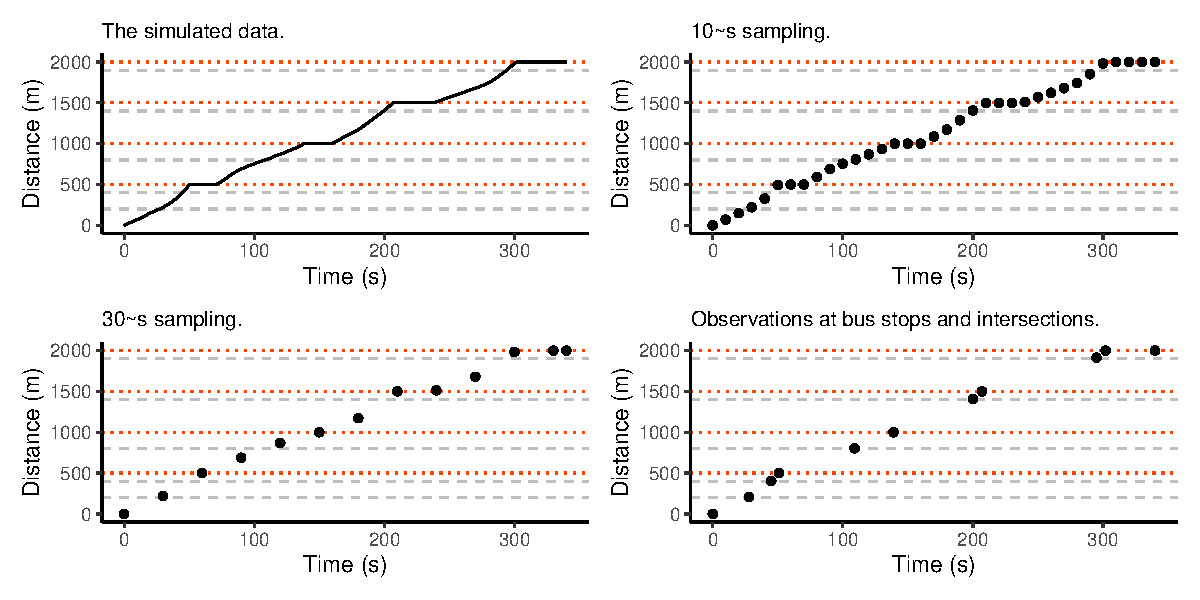
\includegraphics[width=\linewidth]{figure/sim2_graph-1} \caption[Vehicle trajectory with sampled observations for simulation B]{A simulated vehicle trajectory (top left) for simulation B along five road segments (dashed grey lines) with four stops (dotted orange lines) sampled using the three techniques (see text).}\label{fig:sim2_graph}
\end{figure}


\end{knitrout}

\begin{knitrout}\small
\definecolor{shadecolor}{rgb}{0.969, 0.969, 0.969}\color{fgcolor}\begin{figure}[p]
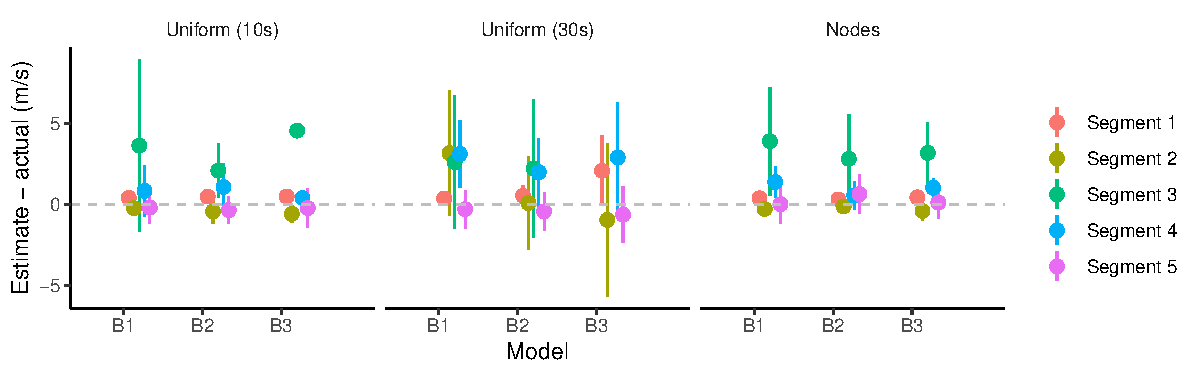
\includegraphics[width=\linewidth]{figure/sim2_pf-1} \caption[Results for simulation B]{Simulation B results for the three models (B1, B2, B3) applied to the data from three sampling methods using $\Np=2000$ particles. Shown is the travel time prediction error along with its standard deviation.}\label{fig:sim2_pf}
\end{figure}


\end{knitrout}





\begin{knitrout}\small
\definecolor{shadecolor}{rgb}{0.969, 0.969, 0.969}\color{fgcolor}\begin{figure}[p]
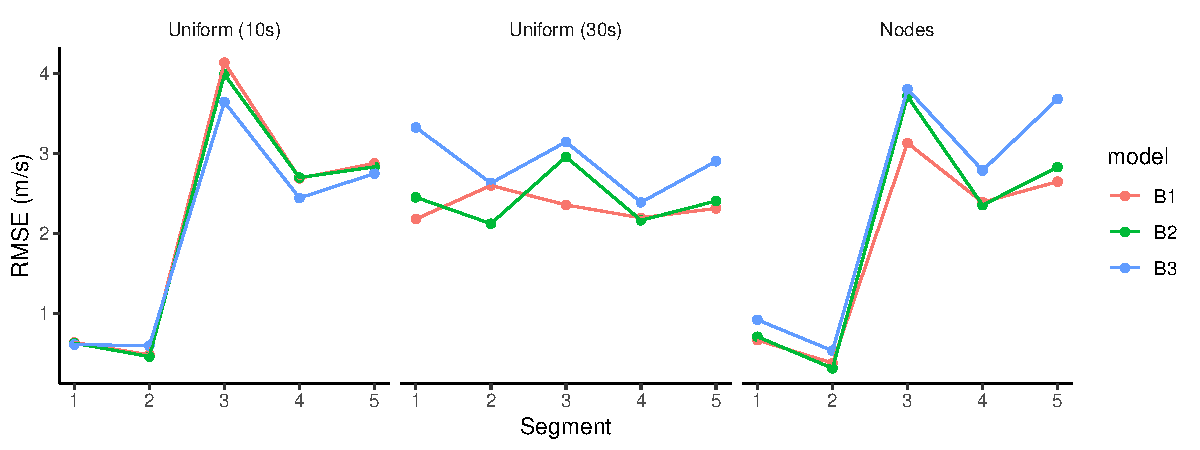
\includegraphics[width=\maxwidth]{figure/sim2_pf_full-1} \caption[Results for simulation B replicated 100~times]{Speed estimation results for 100 simulations. In each the vehicle trajectory was simulated using a different seed and speed estimated by the mean of the particles, which is compared to the true speed using \gls{rmse}.}\label{fig:sim2_pf_full}
\end{figure}

\begin{table}[p]

\caption{\label{tab:sim2_pf_full}RMSE and MAE of average speed estimation for simulation B for three models and three sampling techniques.}
\centering
\fontsize{8}{10}\selectfont
\begin{tabular}[t]{llrr}
\toprule
Sampling method & Model & RMSE (m/s) & MAE (m/s)\\
\midrule
Uniform (10s) & B1 & 2.56 & 1.40\\
 & B2 & 2.51 & 1.35\\
 & B3 & 2.34 & 1.35\\
\midrule
Uniform (30s) & B1 & 2.34 & 1.58\\
 & B2 & 2.43 & 1.63\\
 & B3 & 2.90 & 2.14\\
\midrule
Nodes & B1 & 2.15 & 1.31\\
 & B2 & 2.36 & 1.35\\
 & B3 & 2.70 & 1.57\\
\bottomrule
\end{tabular}
\end{table}


\end{knitrout}





Repeating the simulation 100~times with different vehicle trajectories, we can better compare the models (\cref{fig:sim2_pf_full}). Uncertainties are now much higher, on average, particularly under low-frequency sampling. The models all perform similarly, though B3 has the worst accuracy overall. \Cref{tab:sim2_pf_full} compares the estimates numerically using \gls{rmse} and \gls{mae}, where we see that within each sampling method the errors are similar. Models B1 and B2 perform similarly, while B3 is again consistently worse except under high-frequency sampling.




\phantom{\gls{rmse} \gls{mae}}
